% ~~~~~~~~~~~~~~~~~~~~~~~~~~~~~~~~~~~~~~~~~~~~~~~~~~~~~~~~~~~~~~~~~~~~~~~~~~~~~
%                                 QUORIDOR
% ~~~~~~~~~~~~~~~~~~~~~~~~~~~~~~~~~~~~~~~~~~~~~~~~~~~~~~~~~~~~~~~~~~~~~~~~~~~~~
\chapter{Quoridor}\label{chap:3}
  \lhead{Chapter 3. \emph{Quoridor}}

\section{History}
TODO

\section{Rules}
\begin{wrapfigure}{R}{0.4\textwidth}
  \vspace*{-2.80cm}
  \centering
  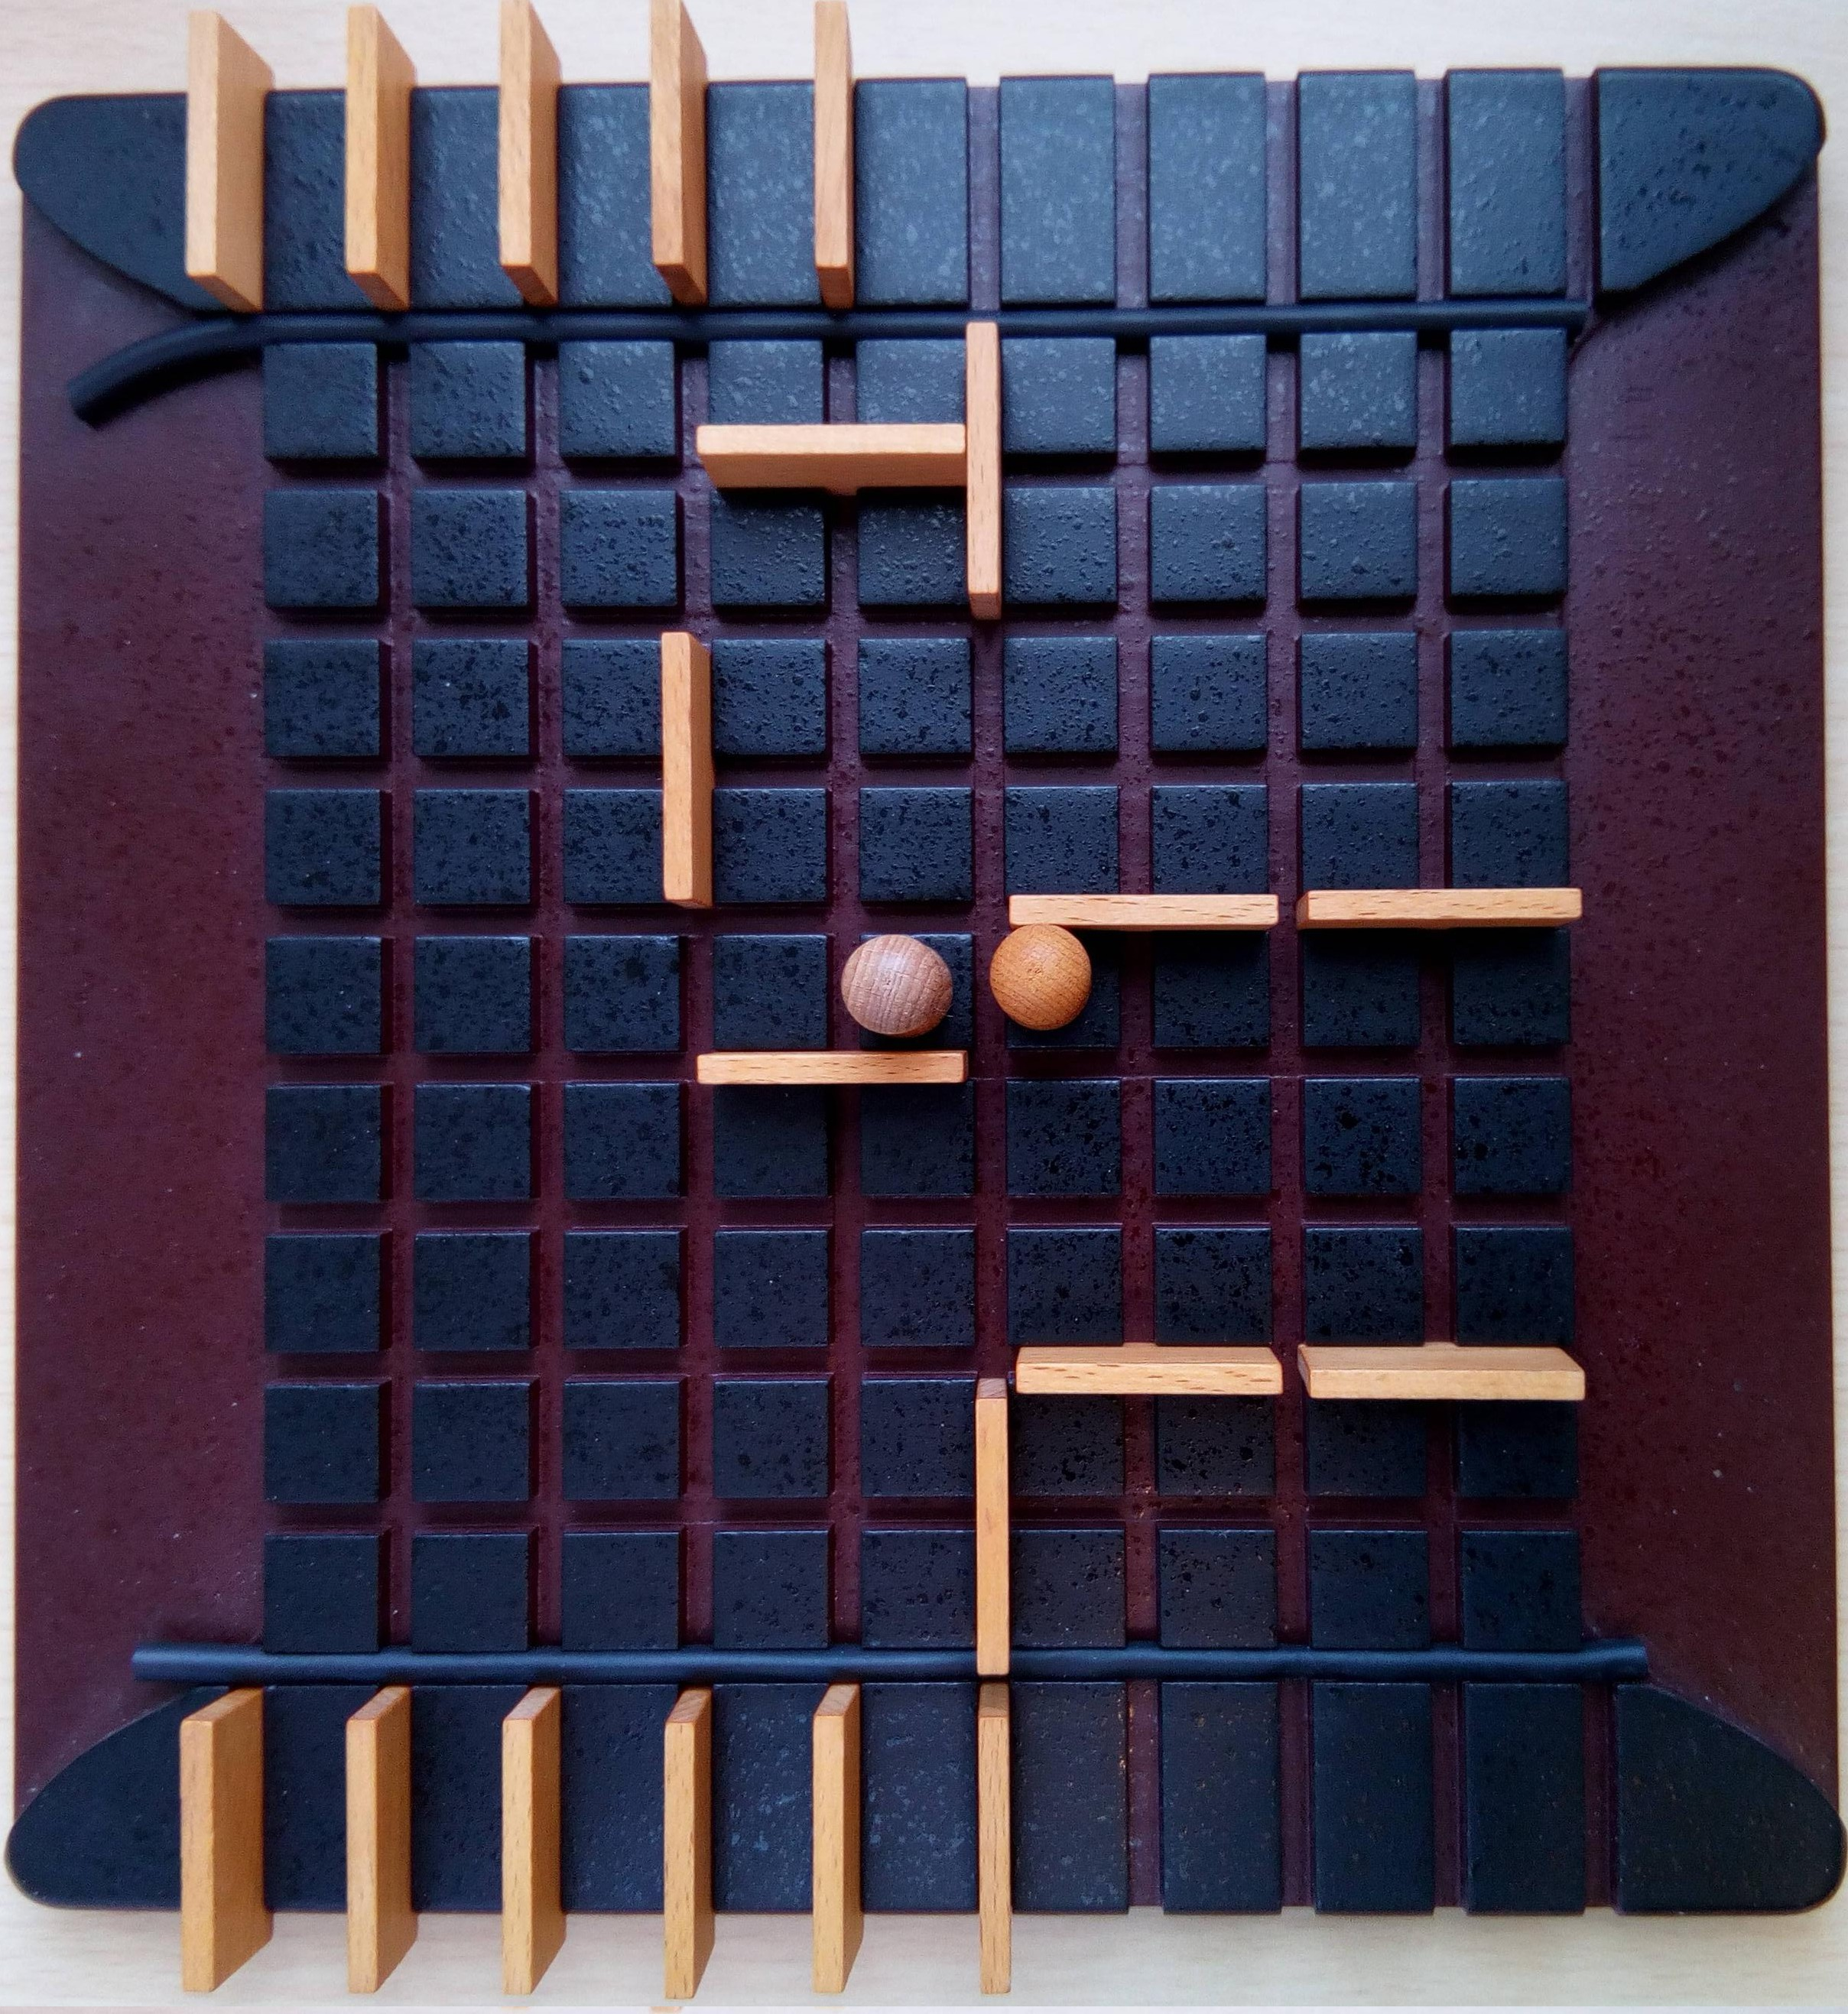
\includegraphics[width=0.35\textwidth]{real_board.jpg}
  \vspace*{-0.60cm}
  \caption{quoridor board}
  \label{fig:quoridor_board}
  \vspace*{-1.00cm}
\end{wrapfigure}

Quoridor is abstract board strategy game for 2 or 4 players with size of
9x9 (81) squares. This thesis covers 2 player version of the game.

Each player starts with a single pawn in the center of the edge on the
opposite side as the opponent.
The goal for each player is to reach the opposite edge.

\begin{wrapfigure}{L}{0.35\textwidth}
  \vspace*{-0.20cm}
  \centering
  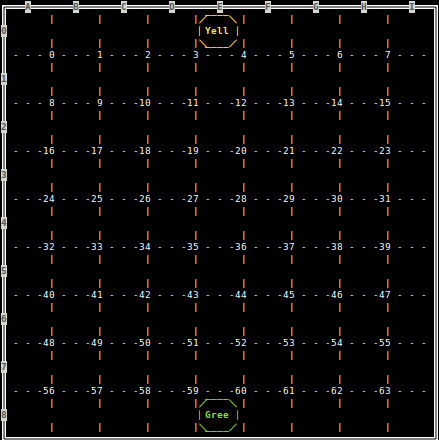
\includegraphics[width=0.35\textwidth]{start.png}
  \vspace*{-1.20cm}
  \caption{game start}
  \label{fig:game_start}
  \vspace*{-0.40cm}
\end{wrapfigure}

Player also starts with 10 walls (fences) in the stock.
Walls are two space wide and can be placed in the groove that runs between
the spaces.
Placed wall blocks pawns paths forcing them to go arount it.
Walls once placed can not be moved nor removed.
Wall can not be placed to the position already occupied or crossing by
other wall.
Also, wall can not cut off the only remaining path of any pawn to his goal.

When player is on turn, he must place wall, if he has left some, or move
his pawn to adjacent (not diagonal and unoccupied) space.
If opponent's pawn stands on an adjacent space, current player can jump
with his pawn to all the places where the opponent pawn can move.

\section{State Complexity}
Estimated game state complexity was $3.9905\cdot10^{42}$
\cite{mertens} (equation \ref{eqn:mertensestimate}), however, this is very rough estimate, since
it includes many states multiple times where it counts with permutations
instead of combinations of walls.

\begin{center}
  \vspace*{-1.30cm}
  \begin{equation}
    \label{eqn:mertensestimate}
    \begin{aligned}
      S_p\!&=\!81 \cdot 80 = 6480 \\
      S_f\!&=\!\sum_{i=0}^{20}\prod_{j=0}^{i}(128 - 4i)\!=\!6.1582{\cdot}10^{38} \\
      S\!&=\!S_p \cdot S_f = \mathbf{3.9905 \cdot 10 ^{42}}
    \end{aligned}
  \end{equation}
  \vspace*{-1.15cm}
\end{center}

My approach (equation \ref{eqn:myestimate}) with estimating state complexity
will be similar. I will estimate maximum states of this game, which will
include impossible states such as:
\begin{itemize}
  \vspace*{-0.25cm}
  \setlength\itemsep{0cm}
  \item walls crossing each other
  \item pawns in the winning position and on turn
  \item pawns not having the path to the winning position
  \item pawn in the winning position where it could not end due to walls
  \vspace*{-0.15cm}
\end{itemize}
Moreover, this estimate will count as a different state when different
player is on the move, and also, different number of walls in players
stocks. Both of these could make the game very different in the outcome.

\begin{center}
  \vspace*{-1.30cm}
  \begin{equation}
    \label{eqn:myestimate}
    \begin{aligned}
      S_p &= 81 {\cdot} 80 - 9 {\cdot} 9 = 6399\\[-0.20cm]
      f(i)\!&=\! \begin{cases}
        i + 1  & \quad \text{if } i <= 10 \\[-0.30cm]
        21 - i & \quad \text{if } i > 10
      \end{cases}\\
      S_f\! &=\! \sum_{i=0}^{20} f(i){128 \choose i} = 1.7796 {\cdot} 10^{23}
      \\
      S &= 2 {\cdot} S_p {\cdot} S_f = \mathbf{2.2775 {\cdot} 10^{27}}
    \end{aligned}
  \end{equation}
  \vspace*{-1.15cm}
\end{center}

$S_p$ was corrected to not include both pawns in the winning positions.
$f(i)$ % is from sequence $\{1, 2, ..., 9, 10, 11, 10, 9, ..., 2, 1\}$ and
stands for different wall counts in the stocks.
$2$ in $2{\cdot} S_p {\cdot} S_f$ represents different players on turn.

The result is maximum number of possible states, which is significantly
less then former estimate. However, even if I could evaluate $10^{6}$
states in one second, it would take around $7.2172{\cdot}10^{13}$ years to
evaluate this many states. Also, lets assume it takes on average 50B
of memory per state. Then I would need approximately
$1.1387{\cdot}10^{29}$ bytes of memory to store all states in the
computer. This is why simple Q-learning is not feasible.

{\color{red}TODO: very precise estimate would be, if we could compute not crossing
positions for each number of placed walls...}

\section{Game Tree Complexity}
Average branging factor of the game has been calculated to be $60.4$ and
average game length to be $91.1$ \cite{glendenning}. Mertens \cite{mertens}
used this to compute game-tree size $G$:
\begin{center}
  \vspace*{-1.30cm}
  \begin{equation}
    \label{eqn:mgtc}
    G = 60.4^{91.1} = 1.7884{\cdot}10^{162}
  \end{equation}
  \vspace*{-1.30cm}
\end{center}

\begin{wrapfigure}{r}{0.38\textwidth}
  \vspace*{-0.45cm}
  \centering
  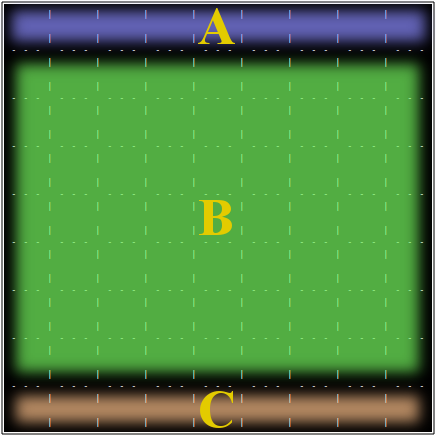
\includegraphics[width=0.35\textwidth]{areas.png}
  \vspace*{-0.60cm}
  \caption{board areas}
  \label{fig:areas}
  \vspace*{-0.60cm}
\end{wrapfigure}

First, I will estimate upper bound of all states where decision can be made.
After this, I will estimate upper bound of all different decisions.
Branching factor will be simply division of these.

To count every possible pawn move, board is divided into three areas
(fig. \ref{fig:areas}), where $A$ and $C$ are positions from the first
and last row respectively and $B$ are positions from $7$ rows from the middle.
So, position AC means, first pawn is in the first row and second pawn is
in the last row or BB means, both pawns are in the middle $7$ rows. Then, for
each pattern (fig. \ref{fig:decisions}), possible positions for making
decision and possible decisions are counted.
% where $P$ represents number of possibilites and $D$ represents number of decisions possible.

\begin{wrapfigure}{H}{0.99\textwidth}
  \vspace*{-12.40cm}
  \centering
  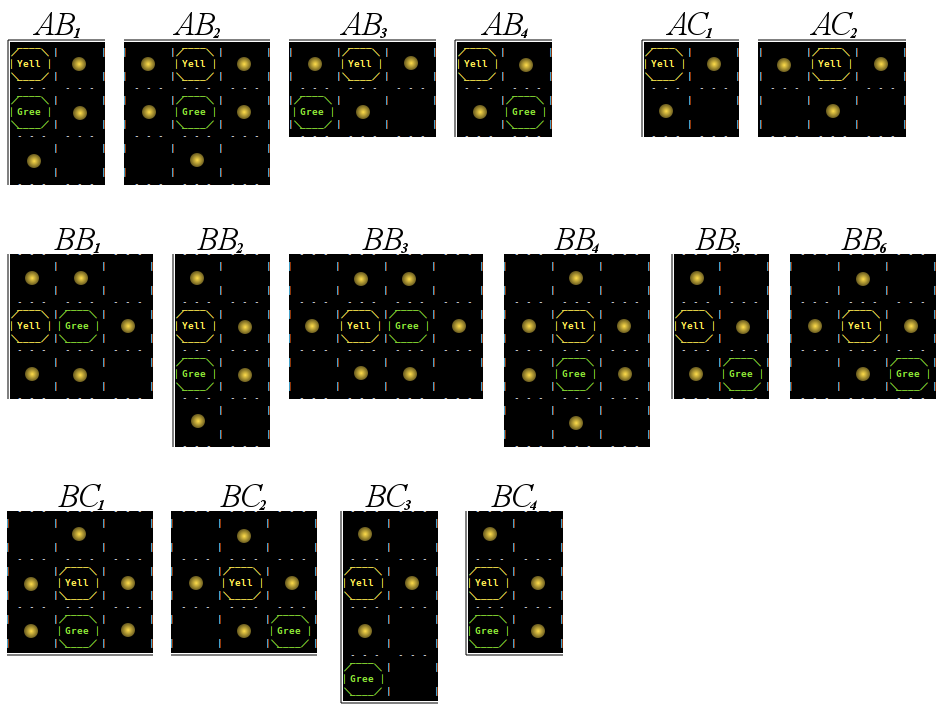
\includegraphics[width=0.95\textwidth]{decisions.png}
  \vspace*{-0.25cm}
  \caption{decission patterns}
  \label{fig:decisions}
  \vspace*{-0.60cm}
\end{wrapfigure}

\vspace{11.70cm}
.

\begin{wraptable}{r}{0.55\textwidth}
  \centering
  \begin{tabular}{| l | r | r |}
    \hline
    & Possitions & Decisions \\ \hline
    $AB_{1}$ & $2$ & $2\cdot3=6$ \\ \hline
    $AB_{2}$ & $7$ & $7\cdot5=35$ \\ \hline
    $AB_{3}$ & $7\cdot62=434$ & $434\cdot3=1302$ \\ \hline
    $AB_{4}$ & $2\cdot62=124$ & $124\cdot2=248$ \\ \hline \hline

    $AC_{1}$ & $2\cdot9=18$ & $18\cdot2=36$ \\ \hline
    $AC_{2}$ & $7\cdot9=63$ & $63\cdot3=189$ \\ \hline \hline

    $BB_{1}$ & $7\cdot2\cdot2=28$ & $28\cdot5=140$ \\ \hline
    $BB_{2}$ & $6\cdot2\cdot2=24$ & $24\cdot4=96$ \\ \hline
    $BB_{3}$ & $6\cdot2\cdot7=84$ & $84\cdot6=504$ \\ \hline
    $BB_{4}$ & $6\cdot2\cdot7=84$ & $84\cdot6=504$ \\ \hline
    $BB_{5}$ & $2\cdot2\cdot60 + 5\cdot2\cdot59=830$ & $830\cdot3=2490$ \\ \hline
    $BB_{6}$ &
      $\displaystyle{7*9\choose2}-\sum_{1<i<6}\!BB_{i}=903$ &
      $903\cdot4=3612$ \\ \hline \hline

    $BC_{1}$ & $7$ & $7\cdot5=35$ \\ \hline
    $BC_{2}$ & $42\cdot9 + 7\cdot8=434$ & $434\cdot4=1736$ \\ \hline
    $BC_{3}$ & $6\cdot9\cdot2 + 2\cdot8=124$ & $124\cdot3=372$ \\ \hline
    $BC_{4}$ & $2$ & $2\cdot2=4$ \\ \hline \hline

    \textbf{Total} & $\textbf{3168}$ & $\textbf{11309}$ \\ \hline
  \end{tabular}
  \vspace*{-0.25cm}
  \caption{positions and decisions}
  \label{tab:positions}
  \vspace*{-0.60cm}
\end{wraptable}
